% Copyright (c) 2023-2026 Oriol Cayon, Delft University of Technology
% SPDX-License-Identifier: Apache-2.0
\documentclass[11pt,a4paper]{article}

\usepackage[margin=2.4cm]{geometry}
\usepackage{graphicx}
\usepackage{amsmath,amssymb}
\usepackage{booktabs}
\usepackage{longtable}
\usepackage{xcolor}
\usepackage{caption}
\usepackage{float}
\usepackage{enumitem}
\usepackage{fancyhdr}
\usepackage[hidelinks]{hyperref}
\usepackage{siunitx}
\sisetup{range-phrase={--},range-units=single}

\graphicspath{{figures/}}

\definecolor{accent}{HTML}{D55E00}
\definecolor{muted}{HTML}{555555}

\captionsetup{font=small,labelfont=bf}
\setlist{itemsep=2pt,parsep=0pt,topsep=3pt}

\pagestyle{fancy}
\fancyhf{}
\fancyhead[L]{\small\textsc{Billow --- trim coupling}}
\fancyhead[R]{\small\thepage}
\renewcommand{\headrulewidth}{0.3pt}

\newcommand{\code}[1]{\texttt{\small #1}}

\title{%
  \vspace{-1.5cm}
  {\Huge\textbf{Coupling Billow to the trim}}\\[6pt]
  {\large The minimum-energy structural model driven against the VSM
   quasi-steady trim}\\[10pt]
  {\normalsize Integration, the modelling inputs it exposed, and first results}
}
\author{Oriol Cayon \\ \small Delft University of Technology}
\date{\today}

\begin{document}
\maketitle
\thispagestyle{fancy}

\begin{abstract}
\noindent
Billow --- the standalone minimum-energy structural library documented in
\code{billow.pdf} --- is now driven against the VSM quasi-steady trim inside
AWETrim's existing coupled loop. This note covers the integration itself, three
properties of the coupled problem that had to be understood before the answer
was physical, two modelling inputs that were simply wrong, and the first
converged results on the TU~Delft V3.

The headline structural result: under trimmed aerodynamic load the wing loses
\SI{2.96}{\percent} of its tip-to-tip span, and it does so by \emph{arcing}
rather than stretching --- the leading-edge arc length is conserved to
\SI{0.21}{\percent} while the arch rise grows \SI{2.4}{\percent}. The six main
struts stay effectively straight (\SIrange{22}{44}{\milli\metre} of sagitta over
\SIrange{2.2}{2.6}{\metre}), which is the behaviour a real inflatable strut has
and which the model only reproduces once the canopy is given its real stiffness.
\end{abstract}

\vspace{0.4em}
\noindent\textcolor{muted}{\small A Markdown version of this document, kept in
step with it, is \code{docs/billow/integration.md}.}

\tableofcontents
\vspace{1em}

%--------------------------------------------------------------------------
\section{Architecture}

The coupling adds one module and reuses everything else.

\begin{center}\small
\begin{tabular}{@{}ll@{}}
\toprule
\code{aerostructural/fem/aerostructural\_coupled\_solver.py} & the coupled loop, \textsc{shared} \\
\code{aerostructural/fem/read\_struc\_geometry\_yaml.py} & the geometry reader, \textsc{shared} \\
\code{aerostructural/fem/aero2struc.py} & the load mapping, \textsc{shared} \\
\code{aerostructural/aerodynamic\_vsm.py} & the trim, \textsc{shared} \\
\code{aerostructural/billow/structural\_billow.py} & \textbf{new} --- the only new physics-facing code \\
\code{scripts/aerostructural/run\_simulation\_BILLOW.py} & \textbf{new} --- the driver script \\
\bottomrule
\end{tabular}
\end{center}

The coupled solver in \code{fem/} is, despite its location, not FEM-specific:
it already dispatched on \code{config["structural\_solver"]} between \code{pss}
and \code{kite\_fem}. Adding Billow was a branch at each of seven dispatch
points, not a copy of its thousand lines. \textbf{Any future backend should do
the same.}

\code{structural\_billow.py} is the only module that imports both
\code{awetrim.structural} and the AWETrim schema. That boundary is deliberate
and load-bearing: the structural package stays free of PSS, VSM and YAML
knowledge, so its element physics can go on being validated against closed-form
solutions independently of anything the coupling does.

\subsection{The coupled loop}

Unchanged from the FEM path except for step~7:

\begin{enumerate}[leftmargin=2em]
  \item structural nodes $\rightarrow$ VSM leading/trailing edge points
  \item \code{body\_aero.update\_from\_points}, bridle-line drag segments rebuilt
  \item VSM quasi-steady trim $\rightarrow$ panel forces, moments, trim state
  \item panel loads $\rightarrow$ structural nodes (\code{aero2struc}, \S\ref{sec:chordwise})
  \item inertial and gravity loads distributed by nodal mass
  \item bridle line drag
  \item \textbf{\code{structural\_billow.run\_billow}} $\rightarrow$ new node positions
  \item Aitken relaxation on the node displacement
  \item tape actuation, if any
  \item convergence check
\end{enumerate}

\subsection{Element mapping}

\code{structural\_billow.instantiate} consumes exactly the arrays
\code{read\_struc\_geometry\_yaml.main} already returns, so one reader serves
both backends.

\begin{center}\small
\begin{tabular}{@{}lll@{}}
\toprule
\textbf{reader element} & \textbf{Billow element} & \textbf{note} \\
\midrule
\code{inflatable\_beam} & \code{InflatableBeamKernel} & diameter in \code{k\_arr}, pressure in \code{c\_arr} \\
\code{pulley} arm pairs & \code{PulleyKernel} & rest length is the \textsc{whole} rope \\
bridle \code{noncompressive} & \code{CableKernel} & tension-only \\
canopy grid springs & \textbf{dropped} & replaced by wrinkling CST membrane triangles \\
\bottomrule
\end{tabular}
\end{center}

Replacing the canopy is the point of the exercise. The FEM canopy is a square
spring net with diagonals: too soft by $1-\nu$ in tension, carrying shear only
as a fourth-order effect of the diagonal stretch, and with no notion of a
biaxial stress state at all. A relaxed (Pipkin) membrane carries the fabric's
real biaxial law and settles into a tension field rather than mesh-scale
crumple. Everything else --- bridle, pulleys, tubes --- is element-for-element
the same as the FEM model, so a Billow-versus-FEM difference is attributable to
the canopy and the solver formulation and to nothing else.

On \code{struc\_geometry\_FEM\_full.yaml}: \textbf{268 nodes, 1098 DOF, 47
cables, 20 pulleys, 97 inflatable tube beams, 378 membrane triangles},
replacing 693 canopy springs. Build under a second; the structural solve costs
\SIrange{2}{5}{\second} per coupled iteration against \SIrange{8}{25}{\second}
of VSM, so the structure is not the bottleneck.

\subsection{Geometry}

Billow requires \code{struc\_geometry\_FEM\_full.yaml}. It is the only file in
the repository carrying \code{strut\_tubes}, \code{leading\_edge\_tubes} and
\code{pressure}; the reduced PSM files are bridle-and-spring only and cannot
feed beams or a canopy mesh.

That choice has a consequence worth stating plainly. FEM\_full has 28
leading-edge nodes, hence 27 sections, so the reachable aero panel counts are
$27n$: \textbf{27, 54, 81, 135}. The wes-quasi-steady campaigns run 45 panels,
but that is $9\times5$ on the PSM geometry and is \emph{not reachable here}. 54
is the adopted default --- nearest to 45 and above the 27/36/45 band
\code{as\_config} records as mesh converged.

%--------------------------------------------------------------------------
\section{Three things that had to be true}

Each was found by looking at the converged shape and asking whether it could be
right. None is a solver bug; all three are properties of the coupled problem
that were invisible in the FEM path.

\subsection{The bridle is not in equilibrium as authored}

The kite YAMLs store \emph{measured} rest lengths against \emph{measured} node
positions, and the two do not agree. On FEM\_full, \code{Br\_main\_1} is
\SI{11.5}{\percent} longer than the distance between the nodes it joins --- at
the real $EA/l_0$ that is \textbf{\SI{88}{\kilo\newton} in one line}. Starting a
coupled run there is starting it from an explosion.

\code{relax\_bridles} settles the bridle onto the held wing before the model is
built: every wing grid node fixed, the KCU pulled down and then settled, the
whole structure re-centred. Peak cable tension \SI{88}{\kilo\newton} $\rightarrow$
\SI{0.4}{\newton}. Because the wing is held, the canopy and tube reference
configurations are untouched up to a rigid translation, which no reference
strain can see.

This is the same role \code{structural\_kite\_fem.relaxbridles} plays on the FEM
path. \textbf{The consequence for callers: the nodes the coupled loop starts
from are not the raw YAML nodes} --- read them back from
\code{structure.model.nodes}.

Related: the reader used to compute the bridle stiffness as $EA/l_0$ and then
discard it for a hard-coded \SI{5000}{\newton\per\metre}, a bridle roughly
$17\times$ too soft. Fixed; the PSS reader had always done it correctly.

\subsection{Reference curvature breaks before the physics does}

The beam's reference curvature is $\omega_0 = \psi / L_0$ with $\psi$ a
Rodrigues vector. It grows like $\tan(\theta/2)$ and is singular at
$\theta = \pi$, so a \emph{short} element bridging a \emph{large} frame change
is numerically hostile long before it is physically wrong.

Seeding each member's roll independently --- the obvious thing --- put the worst
LEI-V3 element at \textbf{\SI{173}{\degree}, $\omega_0 = \SI{753}{\per\metre}$
on a \SI{17}{\milli\metre} element}, seven degrees from the chart singularity.

The fix uses a property of the section rather than a numerical trick. An
inflated tube is isotropic in roll ($GA_2 = GA_3$, a single bending law), so
only $\mathbf{d}_1$ is physically determined and the roll is entirely free.
Spending it on conditioning --- transporting frames by minimal rotation over the
beam tree, and letting the \emph{long} member own each leading-edge/strut joint
(\code{junction\_frame="strut"}: the LE runs are \SIrange{300}{750}{\milli\metre},
the strut stubs \SIrange{17}{97}{\milli\metre}) --- gives
\SI{10.6}{\per\metre}, a factor of 71.

\subsection{A gravity-only load case is not a smoke test}

The KCU is pinned \emph{below} the wing, so gravity alone slackens every bridle
line and the bridle knots become a mechanism. The residual then sits at exactly
their weight --- \SI{2.021}{\newton} on nodes 79 and 113 --- and no amount of
solver tuning moves it.

Billow reports this faithfully. \code{kite\_fem} never shows it because its
\code{I\_stiffness = 25} acts as a ground spring on every node, quietly holding
unsupported nodes up. \textbf{Read a stuck residual equal to some node's load as
``this node has no load path'', not as a conditioning problem.}

%--------------------------------------------------------------------------
\section{Two inputs that were wrong}

\subsection{Apparent wind speed, and the end of self-similarity}
\label{sec:va}

\code{as\_config}'s flight state is zero elevation, zero azimuth,
\SI{90}{\degree} course, gravity off --- the \emph{fastest corner of the wind
window}. At \SI{8}{\metre\per\second} wind and the trimmed $L/D$ of about 4.8
that is $v_a \approx \SI{38}{\metre\per\second}$, above the entire
\SIrange{13}{25}{\metre\per\second} band the wes-quasi-steady campaigns sweep.

For the FEM path this mattered less than it looks, because the campaigns argue
that coupled trims are $v^2$-self-similar and correct for it. \textbf{That
argument does not survive the introduction of the tubes.} The inflatable bending
law
\begin{equation}
  M(\kappa) \;=\; M_{\max}\left(1 - e^{-EI_0\,\kappa / M_{\max}}\right)
\end{equation}
\emph{saturates}. Past $M_{\max}$ the tube has essentially no incremental
bending stiffness and hinges at constant moment --- the compression-side
wrinkling collapse of a real inflated tube. Collapse is reported, not enforced,
because a dropping post-collapse moment would be an unbounded mechanism that
energy minimisation would simply run away from.

A saturating law has no self-similarity: the load decides whether the tubes are
inside their calibrated range at all. At $v_a = \SI{38}{\metre\per\second}$
every strut sat \textbf{\numrange{3.0}{4.7} times past its collapse curvature},
at \SIrange{86}{94}{\percent} of $M_{\max}$, and hinged into
\SIrange{17}{21}{\percent} of chord.

\subsection{Canopy stiffness}
\label{sec:canopy}

The canopy was initially set to $Et = \SI{5000}{\newton\per\metre}$ to match the
kite\_fem spring net, on the reasoning that it made the two canopies
comparable. It made them comparable \emph{and both wrong}: at any plausible
sailcloth thickness \SI{5000}{\newton\per\metre} is $E \approx \SI{20}{\mega\pascal}$,
which is rubber.

The real cloth is already described in the geometry file.
\code{canopy\_density: 170}\,\si{\gram\per\metre\squared} of polyester ripstop
gives a solid-equivalent thickness of $0.170/1380 = \SI{123}{\micro\metre}$, and
at a crimp-derated in-plane modulus of \SI{4}{\giga\pascal} that is
$Et \approx \SI{4.9e5}{\newton\per\metre}$ --- about a hundred times stiffer.

A canopy that soft does not carry load; it billows, and drags the struts with
it. Measured on the same load case, strut sagitta ran
\SIrange{4.5}{6.7}{\percent} of chord at \SI{5e3}{\newton\per\metre} and
\SIrange{0.6}{4.1}{\percent} at \SI{1e6}{\newton\per\metre}.

\begin{quote}\small\color{muted}
The modulus is a \textbf{material estimate, not a measurement}. The repository
contains no tensile data for this cloth. The plausible range ---
\SIrange{2}{12}{\giga\pascal} fibre modulus, varying crimp derating --- spans
$Et$ from \SI{2.5e5}{} to \SI{1.5e6}{\newton\per\metre}. A tensile test on the
actual canopy would replace it, and should.
\end{quote}

%--------------------------------------------------------------------------
\section{Chordwise load placement is the local pitching moment}
\label{sec:chordwise}

Independent of Billow, but surfaced by it, and it changes the FEM path too.

\code{aero2struc} spreads each spanwise VSM panel force over ten chordwise
nodes. \textbf{Where it puts the resultant is the panel's local pitching
moment}, and the wing's trim is a moment balance --- so this is a first-order
modelling choice, not a detail of interpolation.

The historical \code{cp\_file} mode reads one measured $\Delta C_p$ shape from a
single-angle file and applies it to every panel at every angle of attack. Its
centroid on the LEI-V3 file is $0.291c$. Measured on one trim at 135 panels, the
panels' actual centres of pressure --- which VSM already computes from each
panel's own force and moment --- run \numrange{0.303}{0.805}$c$. The fixed
station therefore imposes \textbf{\SI{917}{\newton\metre}} of spurious pitching
moment, about \SI{-10}{\newton\metre} on nearly every panel \emph{with the same
sign}. A systematic bias is precisely what shifts a moment balance; a random one
would largely cancel.

\code{chordwise\_distribution: moment\_matched} keeps the measured shape as a
prior and tilts it onto each panel's own centre of pressure,
\begin{equation}
  w_i \;=\; \frac{w^0_i\,e^{\lambda t_i}}{\sum_j w^0_j\,e^{\lambda t_j}},
  \qquad \sum_i w_i t_i = t_{\mathrm{cp}},
\end{equation}
solving the scalar equation for $\lambda$. Three properties make the exponential
tilt the right correction rather than, say, a least-squares one: every weight
stays strictly positive, so no unphysical negative patch of load appears; the
weights still sum to one, so the panel force is preserved exactly; and $\lambda$
is the natural parameter of an exponential family, whose mean is strictly
increasing in it, so the root exists, is unique, and Newton converges from zero.
It is also the minimum-relative-entropy correction, so the measured shape is
kept wherever the moment does not contradict it.

Residual moment error: \SI{917}{\newton\metre} $\rightarrow$
\SI{6e-9}{\newton\metre}. The default stays \code{cp\_file} so stored results
reproduce; the Billow script sets \code{moment\_matched}.

\begin{figure}[H]
  \centering
  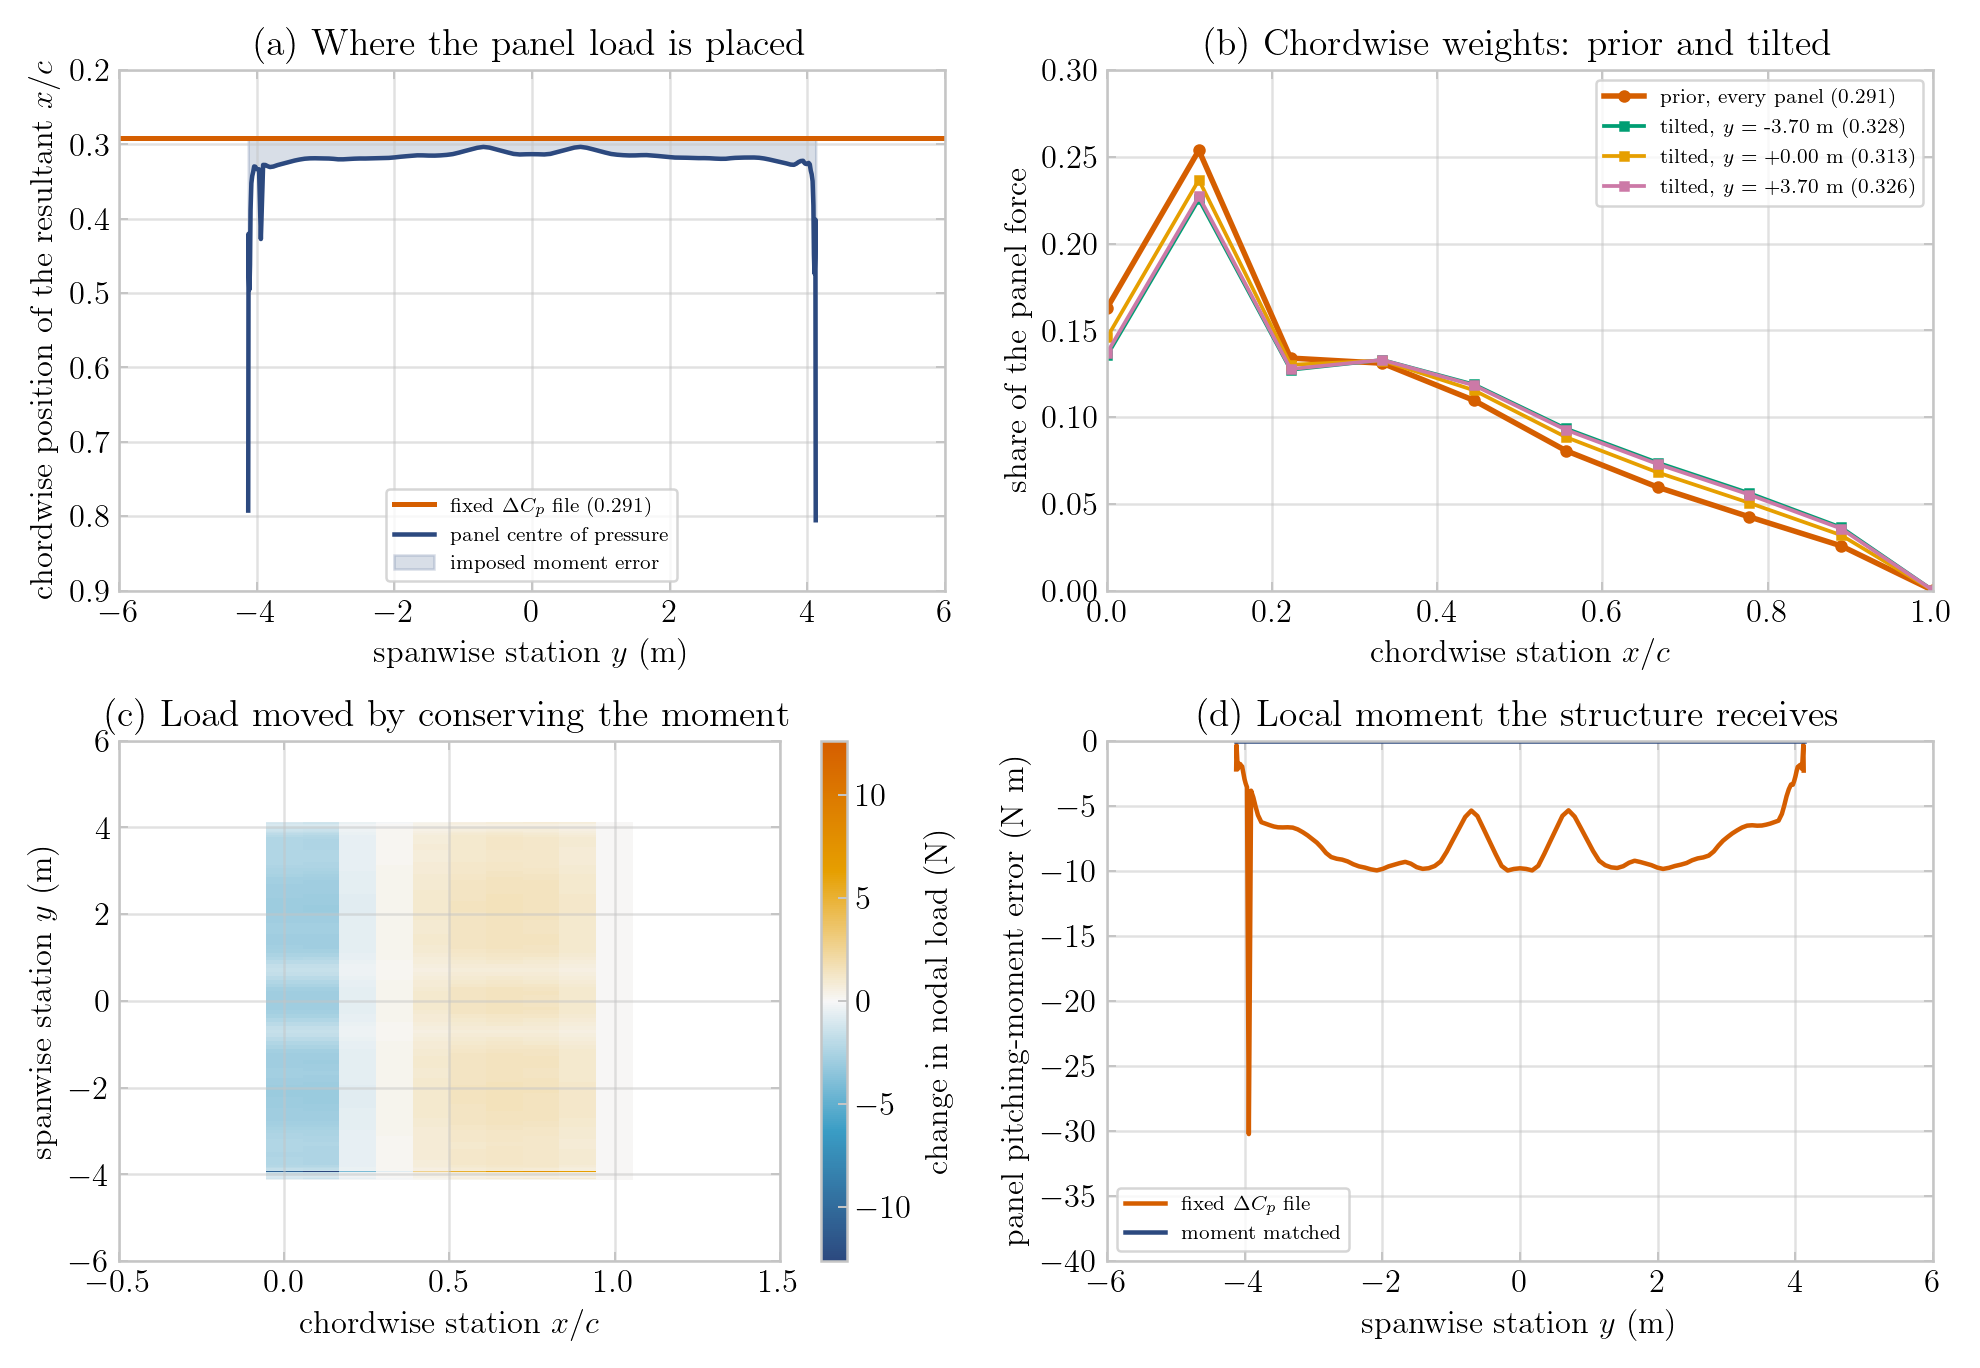
\includegraphics[width=\textwidth]{chordwise_moment_matching.png}
  \caption{Conserving the panel pitching moment. \textbf{(a)} the single fixed
  chordwise station the $\Delta C_p$ file imposes against each panel's actual
  centre of pressure --- the shaded gap is moment the structure receives but the
  aerodynamics never produced; the excursions at $y \approx \pm 4$\,m are the
  stalled tip panels. \textbf{(b)} the prior and three tilted weight sets.
  \textbf{(c)} the load the correction moves: forward of $0.2c$ and aft into
  $0.4$--$0.9c$. \textbf{(d)} the resulting per-panel moment error, about
  $-10$\,N\,m on nearly every panel with the same sign, which is what makes it
  bias a trim, against zero for the matched weights.}
  \label{fig:chordwise}
\end{figure}

\paragraph{A warning about the diagnostic.}
\code{check\_moment\_preservation} does \emph{not} measure any of the above.
Both of its call sites hand it the already-distributed loads, so it reports the
error of the \emph{spatial} nearest-node step alone. That error is
\SI{0.09}{\percent} on the built shape but around \SI{20}{\percent} once the
kite has deformed --- a separate and still-open defect. Do not quote its numbers
as evidence about the chordwise placement.

%--------------------------------------------------------------------------
\section{Preliminary results}

LEI-V3, unactuated (the tape lengths the geometry stores: \code{depower\_tape}
$l_0 = \SI{1.9}{\metre}$, i.e.\ $u_{dp} \approx 0.28$), 54 aero panels, gravity
off, moment-matched chordwise loads, $v_a \approx \SI{24}{\metre\per\second}$.

\subsection{Convergence}

\begin{center}\small
\begin{tabular}{@{}lcc@{}}
\toprule
\textbf{state} & \textbf{iterations} & \textbf{final residual} \\
\midrule
real canopy, $v_a\,24$ & \textbf{2} & \SI{3.84}{\newton} \\
soft canopy, $v_a\,38$ & 7 & \SI{4.33}{\newton} \\
soft canopy, $v_a\,38$, 135 panels & 10 & \SI{4.45}{\newton} \\
\bottomrule
\end{tabular}
\end{center}

Gate is \SI{5}{\newton} absolute. The physically correct case is also by far the
easiest to converge --- worth noting, because a model driven outside its
calibrated range does not merely give a wrong answer, it costs more to get it.

\begin{figure}[H]
  \centering
  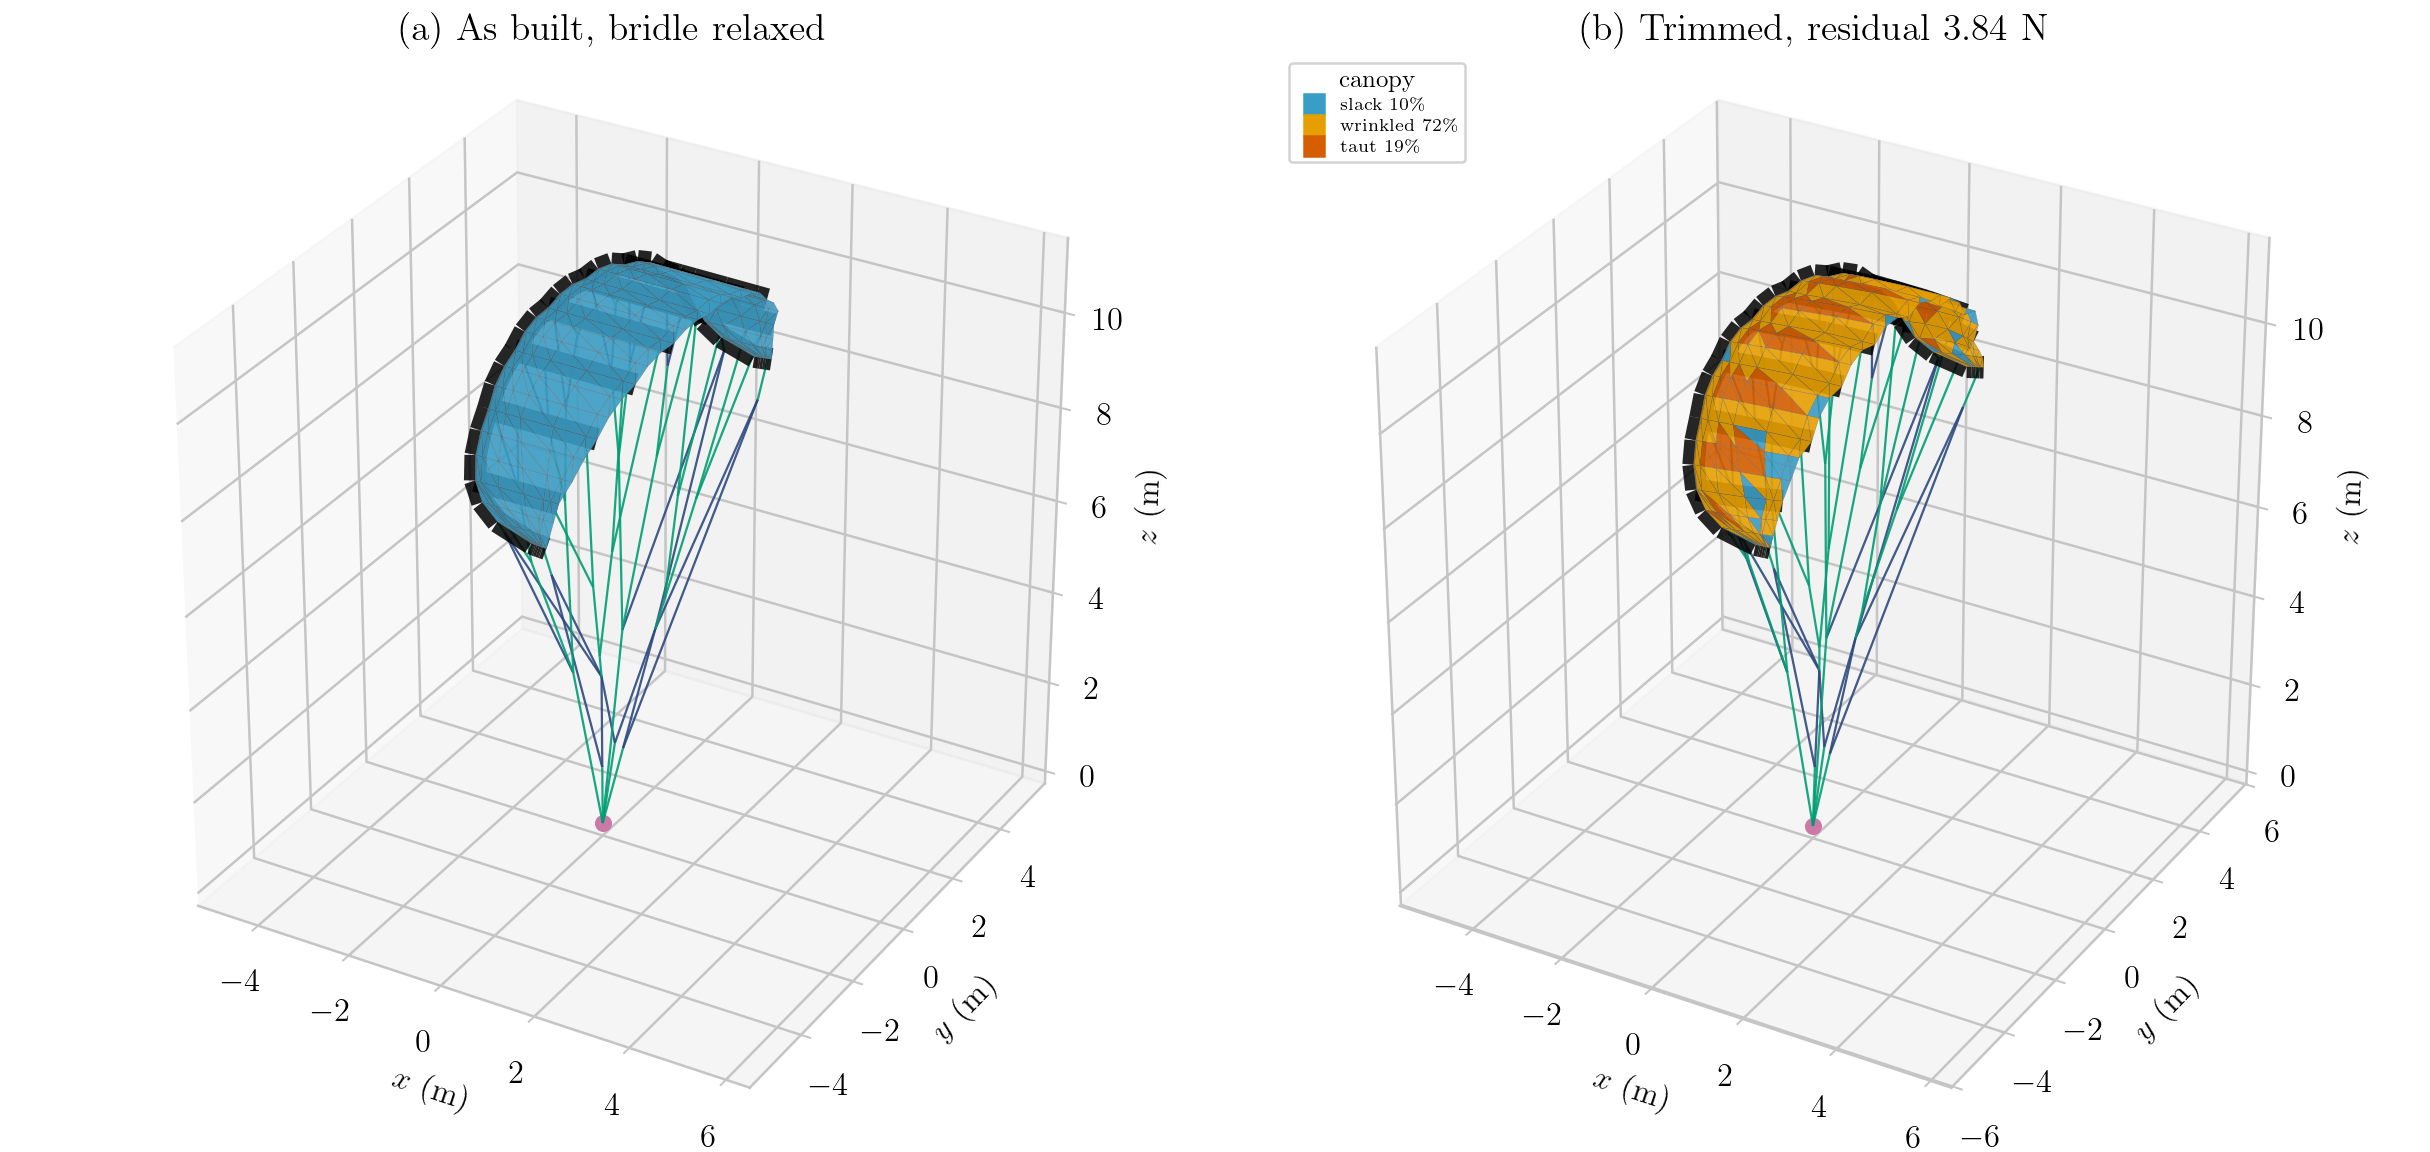
\includegraphics[width=\textwidth]{billow_geometry.png}
  \caption{The first converged coupled solve. \textbf{(a)} the built shape after
  the bridle relaxation of \S2.1, before any aerodynamic load; \textbf{(b)} the
  trimmed shape, canopy shaded by the wrinkling state the solver chose. Black:
  inflatable tubes, drawn at their real relative diameters. Green: bridle
  cables. Blue: pulley ropes through their sheaves. The magenta marker is the
  KCU, the only pinned node.}
  \label{fig:geometry}
\end{figure}

\subsection{Span reduction}

Tip-to-tip is the straight distance between the two leading-edge tips; LE arc is
the length measured along the tube.

\begin{center}\small
\begin{tabular}{@{}lccc@{}}
\toprule
 & \textbf{as built} & \textbf{trimmed} & \textbf{change} \\
\midrule
\textbf{tip-to-tip span} & \SI{8.202}{\metre} & \textbf{\SI{7.959}{\metre}} & \textbf{\SI{-0.243}{\metre}, \SI{-2.96}{\percent}} \\
leading-edge arc length & \SI{12.662}{\metre} & \SI{12.636}{\metre} & \SI{-0.026}{\metre}, \SI{-0.21}{\percent} \\
arch rise above the tip chord & \SI{3.282}{\metre} & \SI{3.362}{\metre} & \SI{+2.42}{\percent} \\
mean chord & \SI{2.044}{\metre} & \SI{2.036}{\metre} & \SI{-0.4}{\percent} \\
\bottomrule
\end{tabular}
\end{center}

\textbf{The span reduces by \SI{3.0}{\percent}, and it does so by arcing, not by
stretching.} The leading-edge arc length is conserved to
\SI{0.21}{\percent} --- the tube neither extends nor compresses --- while the
arch rise grows \SI{2.4}{\percent}. The wing bends into a deeper arc under load
and pulls its tips inward. That is the correct physical picture for a
leading-edge-inflatable kite, and it is a stringent check on the beam
formulation: an axially sloppy beam would have shown span loss through
shortening instead.

For contrast, the same kite with the soft canopy at $v_a = 38$ gives the
\textbf{wrong sign}: tip-to-tip \SI{+2.24}{\percent}, arch rise
\SI{-3.87}{\percent}, mean chord \SI{-7.1}{\percent}, LE arc unchanged. A canopy
at \SI{20}{\mega\pascal} stretches instead of carrying load, so the sail draws
the trailing edge toward the leading edge while the wing \emph{flattens} and
splays its tips outward. Both the sign of the span change and the magnitude of
the chord change are unphysical. This is the clearest single argument for
\S\ref{sec:canopy}.

\subsection{Strut bending}

Sagitta is the maximum perpendicular deviation from the straight line joining
the strut's two ends. Utilisation is curvature over the law's collapse
curvature; above 1.0 the tube is outside the range the ASKITE fits were
calibrated over.

\begin{center}\small
\begin{tabular}{@{}lll@{}}
\toprule
\textbf{configuration} & \textbf{main struts (6)} & \textbf{outboard struts (2)} \\
\midrule
$v_a\,38$, canopy \SI{5}{\kilo\newton\per\metre} & \SIrange{17}{21}{\percent}, \numrange{3.0}{4.7}$\times$ & --- \\
$v_a\,21$, canopy \SI{5}{\kilo\newton\per\metre} & \SIrange{7.1}{9.5}{\percent}, \numrange{1.2}{2.2}$\times$ & --- \\
\textbf{$v_a\,24$, canopy \SI{493}{\kilo\newton\per\metre}} & \textbf{\SIrange{1.0}{1.8}{\percent} (\SIrange{22}{44}{\milli\metre}), \numrange{0.17}{0.25}$\times$} & \SIrange{6.6}{6.8}{\percent}, $1.6\times$ \\
\bottomrule
\end{tabular}
\end{center}

The six main struts are effectively straight --- tens of millimetres over
\SIrange{2.2}{2.6}{\metre} --- and sit comfortably inside the calibrated range.
This matters because real LEI struts do not visibly bend in flight, and a model
that bends them is wrong whatever its residual says.

The two outboard struts remain past collapse. They are the thinnest
(\SIrange{0.080}{0.106}{\metre} against \SIrange{0.108}{0.141}{\metre}) and the
shortest, and they sit next to the tip region where VSM reports stall, so they
are where the inflation pressure matters most.

\begin{figure}[H]
  \centering
  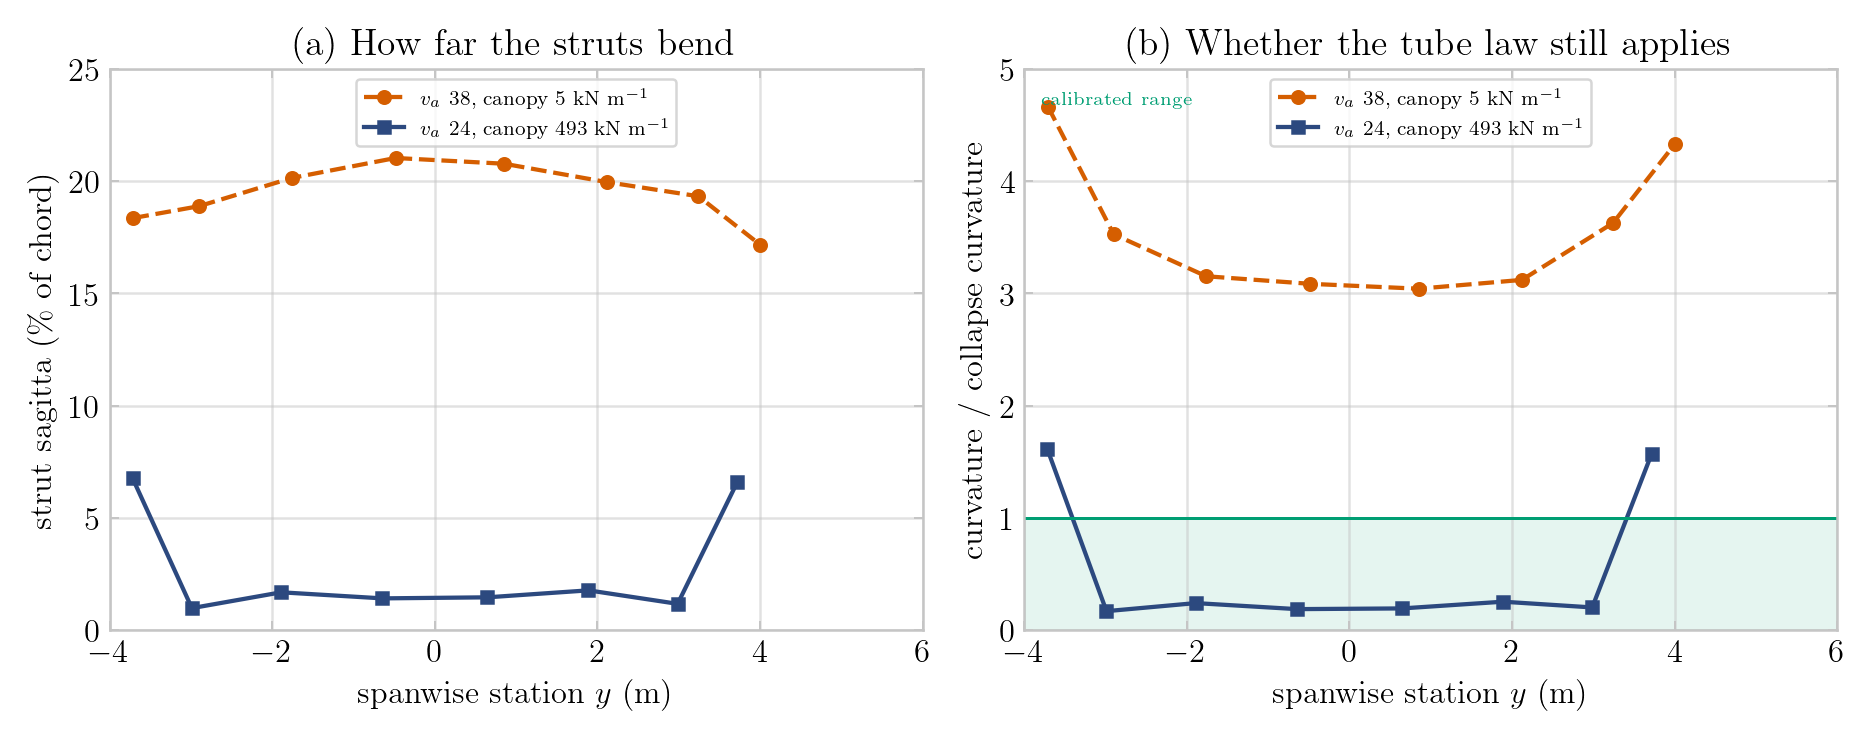
\includegraphics[width=\textwidth]{billow_strut_bending.png}
  \caption{Strut bending along the span. \textbf{(a)} sagitta as a fraction of
  chord; \textbf{(b)} curvature over the collapse curvature of the fitted tube
  law, with the calibrated range shaded. At $v_a\,38$ with the spring-net canopy
  every strut is far outside the range the ASKITE fits cover, so the saturated
  moment leaves them hinging. With the real apparent speed and the real cloth
  the six main struts fall to a fifth of collapse curvature and bend by tens of
  millimetres; only the two thin outboard struts, next to the stalled tip,
  remain above~1.}
  \label{fig:struts}
\end{figure}

\subsection{Canopy state}

Fraction of the 378 membrane triangles in each regime at the solved state.

\begin{center}\small
\begin{tabular}{@{}lcccc@{}}
\toprule
 & \textbf{slack} & \textbf{wrinkled} & \textbf{taut} & \textbf{resultant aero load} \\
\midrule
real canopy, $v_a\,24$ & \SI{9.5}{\percent} & \SI{72.0}{\percent} & \SI{18.5}{\percent} & \SI{3.57}{\kilo\newton} \\
soft canopy, $v_a\,38$ & \SI{1.9}{\percent} & \SI{41.0}{\percent} & \SI{57.1}{\percent} & \SI{10.73}{\kilo\newton} \\
\bottomrule
\end{tabular}
\end{center}

The realistic canopy is predominantly \textbf{wrinkled} --- carrying tension in
one direction and none across it. That is the expected state for a sail: a
genuine tension field over most of the surface, going taut only where it is
pulled biaxially. The soft canopy at three times the load reads as mostly taut
simply because it has stretched far enough to carry biaxial tension everywhere,
which is what a rubber sheet would do.

This diagnostic has no counterpart in the spring-net canopy. A net has no
biaxial stress state and so cannot distinguish these cases at all.

\subsection{Depower sweep}

Continuation chains either side of the built tape length, at three winds:
26 converged points over $u_{dp} = \numrange{0.243}{0.314}$, in
19 minutes. Each chain walks the tape inside a single coupled call so every step
warm-starts the next; the alternative, solving each point independently, was
measured at 14 minutes \emph{per point}.

\begin{figure}[H]
  \centering
  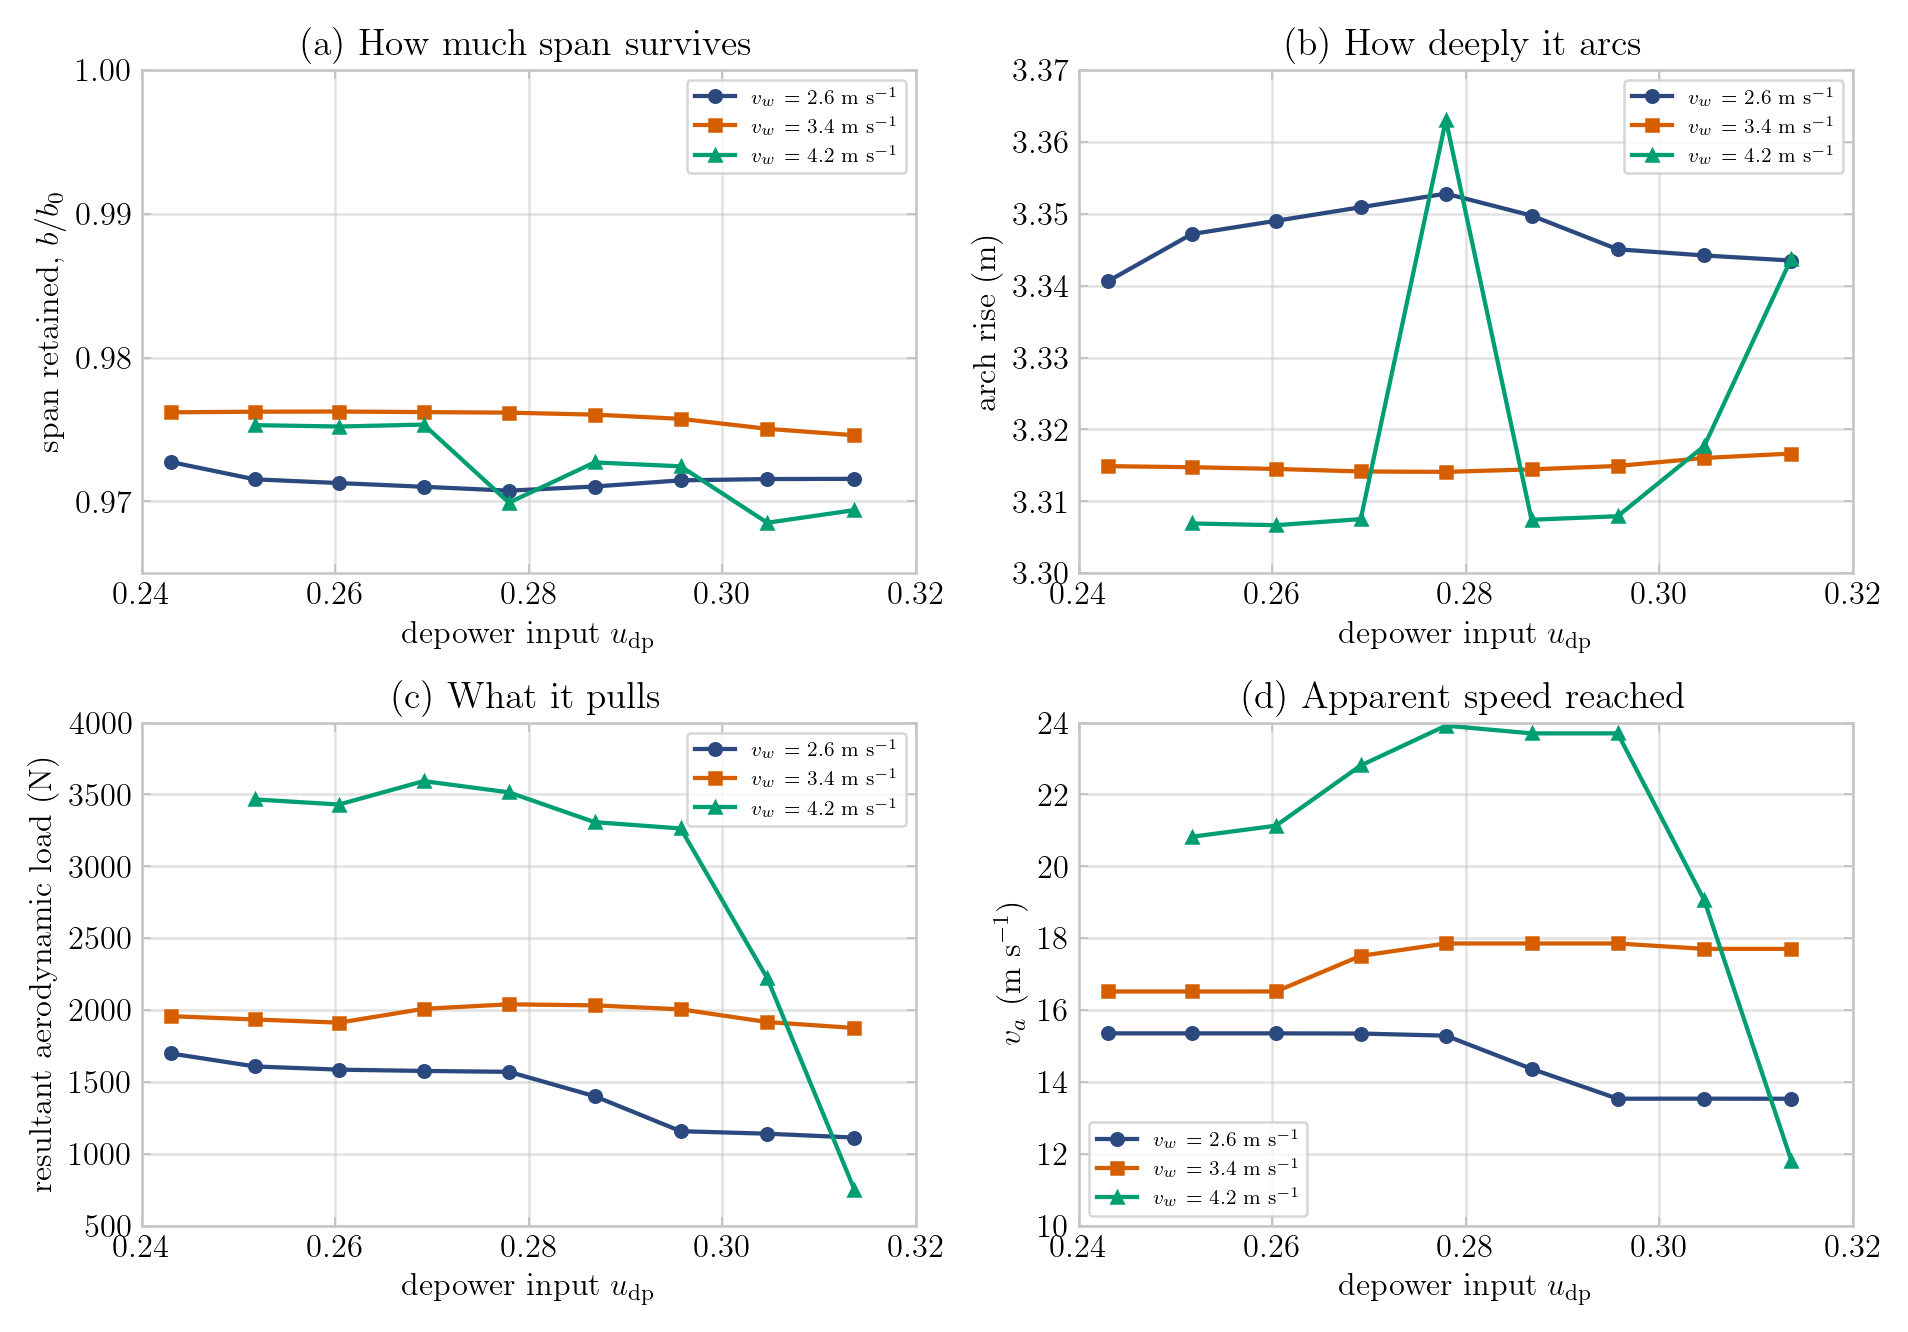
\includegraphics[width=\textwidth]{depower_chains.png}
  \caption{Depower chains at the window centre. Each curve is one wind speed;
  within a chain the wind is held, so $v_a$ slides with $u_{dp}$ and panel
  \textbf{(d)} is a readout rather than a control. \textbf{(a)} span retained
  against the as-built \SI{8.202}{\metre}. \textbf{(b)} arch rise --- the
  outlier at $u_{dp}=0.278$ is the built point, the only step in each chain
  without a warm start. \textbf{(c)} resultant aerodynamic load. The
  $v_w=\SI{4.2}{\metre\per\second}$ curve leaves the attached branch past
  $u_{dp}\approx0.30$ in both \textbf{(c)} and \textbf{(d)}.}
  \label{fig:depower}
\end{figure}

\textbf{Span loss is nearly invariant over the box.} Between \SI{96.9}{\percent}
and \SI{97.6}{\percent} of the built span is retained everywhere in the grid:
depowering by 0.07 in $u_{dp}$ and nearly doubling the wind barely move it. The
\SI{2.96}{\percent} of \S5.2 is therefore the wing's signature across this
operating box rather than a property of one trim point.

\textbf{What depower controls is load, not shape.} The resultant aerodynamic
force falls \SI{29}{\percent} at $v_w=\SI{2.6}{\metre\per\second}$ and
\SI{35}{\percent} at \SI{3.4}{\metre\per\second} across the $u_{dp}$ range,
against about \SI{0.5}{\percent} of span movement. At least this far from stall,
the depower tape is a load knob.

Three caveats, all visible in the figure and none yet resolved:

\begin{enumerate}[leftmargin=2em]
  \item \textbf{The highest-wind chain leaves the attached branch} past
    $u_{dp}\approx0.30$: load \SIrange{3263}{751}{\newton}, $v_a$
    \SIrange{23.7}{11.8}{\metre\per\second}. At $u_{dp}=0.314$ the highest wind
    pulls \emph{less} than the lowest, which is deep stall rather than depower.
    Those points want the attached-branch guard the campaign scripts use.
  \item \textbf{The built point of each chain is under-converged}, being the one
    step with no warm start (\SI{4.11}{\newton} against about
    \SI{2}{\newton}); it is the arch-rise outlier in panel~(b). An artifact of
    chain structure, not physics.
  \item \textbf{Span is not monotonic in wind} --- \SI{2.6}{\metre\per\second}
    loses more span than \SI{3.4}{\metre\per\second}. Unexplained; it may be
    caveat~2 leaking in.
\end{enumerate}

The flat $v_a$ segments in panel~(d) are \code{quasi\_steady\_trim.max\_nfev: 8}:
the warm-started trim returns a bit-identical \code{opt\_x} when it starts inside
tolerance, so $v_a$ repeats exactly. Harmless, but $v_a$ per step is not
independently converged.

%--------------------------------------------------------------------------
\section{Open items}

\begin{enumerate}[leftmargin=2em]
  \item \textbf{Strut inflation pressure.} \code{struc\_geometry\_FEM\_full.yaml}
    records \code{pressure: 0.3}\,bar, which sets both $M_{\max}$ and $EI_0$
    through the ASKITE fits. The two outboard struts are still $1.6\times$ past
    collapse, and being the thinnest they are the most pressure-sensitive
    members on the kite. The real V3 operating pressure should be confirmed.
  \item \textbf{Canopy modulus is an estimate} (\S\ref{sec:canopy}). Its
    plausible range is roughly $\pm3\times$, and the results are sensitive to it
    --- including the \emph{sign} of the span change at the soft end.
  \item \textbf{The spatial load mapping loses moment.}
    \code{map\_aero\_forces\_to\_struct\_nodes} drops ${\sim}\SI{20}{\percent}$
    of the applied moment once the kite has deformed
    (\S\ref{sec:chordwise}). The chordwise placement is now exact; this step is
    not.
  \item \textbf{Tube axial and shear stiffness are derived, not fitted.} The
    ASKITE fits cover bending and torsion only; $EA$ and $\kappa GA$ are read
    off the same fits' initial slopes as a modulus over the thin-wall section.
    Defensible and not a sensitive quantity, but an assumption.
  \item \textbf{The stiffness ladder is untested end to end.}
    \code{set\_stiffnesses} exists and is unit-tested, but no coupled run has
    used a stiffness continuation ramp the way the PSS path does.
  \item \textbf{Steering and depower actuation are wired but unexercised.}
\end{enumerate}

%--------------------------------------------------------------------------
\section{Running it}

\begin{verbatim}
python scripts/aerostructural/run_simulation_BILLOW.py
\end{verbatim}

Results land in \code{results/<kite>/aerostructural/billow/<case>/} as
\code{sim\_output.h5} plus the deformed structural and aerodynamic geometry
YAMLs. The results directory is keyed on actuation only and is
\textbf{overwritten} between runs that differ in anything else --- copy a run
aside before changing panel count, wind or canopy stiffness.

Numerics live in the \code{structural\_billow} block of \code{as\_config.yaml};
every key is listed with its default in \code{structural\_billow.DEFAULTS}, and
unknown keys are rejected rather than ignored. Two diagnostics:

\begin{verbatim}
python scripts/aerostructural/plot_billow_geometry.py
python scripts/aerostructural/plot_chordwise_moment_matching.py
\end{verbatim}

A depower sweep is a pair of continuation chains per wind, walking the tape
either side of its built length and converging at every step:

\begin{verbatim}
python scripts/aerostructural/run_chain_depower_BILLOW.py --wind 2.6 3.4 4.2
python scripts/aerostructural/plot_billow_depower_chains.py
\end{verbatim}

\noindent That writes \code{chains.csv} and one \code{sim\_output.h5} per chain
under \code{results/<kite>/aerostructural/billow\_depower\_chains/}. Each row
carries a \code{converged} flag: a step that missed the residual gate is
recorded rather than dropped, so a short chain cannot read as a complete one.
\code{run\_sweep\_depower\_BILLOW.py} solves each point independently instead
and iterates the wind onto a target apparent speed --- about twenty times more
expensive, and worth it only when a few points must sit at an exact $v_a$.

\code{sim\_output.h5} now stores the nodal material frames alongside the
positions (\code{setup\_tracking\_arrays(..., with\_frames=True)}). A
geometrically exact beam's curvature lives in the frames, not in the node
positions, so without them a saved run cannot afterwards be asked how bent its
tubes were or whether they had passed collapse --- which is exactly the question
the strut results turn on.

\end{document}
